% chktex-file 1
% chktex-file 8
% chktex-file 24
% chktex-file 36
% chktex-file 44

\chapter{Quelltexte}


\begin{minted}[frame=single, framesep=2pt, linenos, fontsize=\tiny, style=vs]{typescript}
export type format = "xml" | "json";
export type mode = "quick" | "detail";
export type sampling = "false" | "primary" | "secondary";
export type diagramResponse = {model?: string, text?: string; xml?: string; json?: DiagramJson | string; 
                               threadId?: string, samples?: {}};
export type modelPriority = Record<format, number>;

export abstract class Ai {
  private createDebugFile: boolean = PRODUCTION.toLowerCase() == "false";

  public model: string = "";
  public format: format = "xml";

  protected constructor(model?: string, format?: format) {
    this.model = model ?? this.model;
    this.format = format ?? this.format;
  }

  public async createBPMN(prompt: string, file: string, userID: number, res: Response, mode: mode = "quick", 
                          stream = false, sampling: sampling = "false"): Promise<diagramResponse> {
    const threadID = await this.createThread();
    const instructions = Array.prototype.concat(Ai.formatInstructions(this.format), Ai.modeInstructions(mode))
    const promptInput = new PromptInput(instructions, prompt, await Ai.getAllChatsFromDB(threadID), null, file);
    const input = this.mapPromptInput(promptInput, mode, stream);
    if (!input) throw new Error("Unable to create input for the ai");
    Ai.getMeasurements(threadID);
    Ai.startStopwatches(['api-response', 'full-response'], threadID)
    const response = await this.generateContent(input, mode, stream);
    Ai.endStopwatch('api-response', threadID)
    if (!response) throw new Error("Ai unreachable");
    const diagramOutput = this.isStream(response)
      ? await this.startStream(response, res, threadID, mode, sampling)
      : await this.startResponse(response, res, threadID, mode, sampling);
    Ai.endStopwatch('full-response', threadID)
    if (!diagramOutput) throw new Error("The ai response is not valid");
    const titleInstructions = "[no prose] [only return title] Find a fitting title for the given scenario";
    const chatTitle = await this.createTitle(`${titleInstructions}\n\n${prompt}`);
    if (!chatTitle) throw new Error("Unable to create title for the thread");
    Ai.startStopwatch('database-save', threadID)
    if (sampling !== "secondary")
      await Ai.saveNewThreadToDB(threadID, userID, chatTitle, prompt, diagramOutput);
    Ai.endStopwatch('database-save', threadID)
    if (sampling === "false" && stream) {
      res.write(`event: save\ndata: success\n\n`);
      res.end();
    } else if (sampling === "false") {
      res.status(201).json(Ai.diagramOutputToStringVersion(diagramOutput));
    }
    return diagramOutput;
  }

  public async updateBPMN(prompt: string, file: string, threadID: string, res: Response, mode: mode = "quick", 
                          stream = false, sampling: sampling = "false"): Promise<diagramResponse> {
    const instructions = Array.prototype.concat(Ai.formatInstructions(this.format), Ai.modeInstructions(mode), await Ai.updateInstructions(threadID, this.format))
    const promptInput = new PromptInput(instructions, prompt, await Ai.getAllChatsFromDB(threadID), undefined, file);
    const input = this.mapPromptInput(promptInput, mode, stream);
    if (!input) throw new Error("Unable to create update input for the ai");
    const response = await this.generateContent(input, mode, stream);
    if (!response) throw new Error("Ai unreachable");
    const diagramOutput = this.isStream(response)
      ? await this.startStream(response, res, threadID, mode, sampling)
      : await this.startResponse(response, res, threadID, mode, sampling);
    if (!diagramOutput) throw new Error("The ai response is not valid");
    if (sampling !== "secondary")
      await Ai.saveUpdatedThreadToDB(threadID, prompt, diagramOutput);
    if (sampling === "false" && stream) {
      res.write(`event: save\ndata: success\n\n`);
      res.end();
    } else if (sampling === "false") {
      res.status(201).json(Ai.diagramOutputToStringVersion(diagramOutput));
    }
    return diagramOutput;
  }

  protected async createThread(): Promise<string> {
    return crypto.randomUUID();
  }

  protected abstract generateContent(input: any, mode: mode, stream: boolean): Promise<any>;

  protected abstract createTitle(prompt: string): Promise<string>;

  public abstract getModelNamesWithPriority(): Map<string, modelPriority>;

  get modelPriority(): number {
    switch (this.format) {
      case "xml": return this.getModelNamesWithPriority().get(this.model)?.xml ?? -1;
      case "json": return this.getModelNamesWithPriority().get(this.model)?.json ?? -1;
      default: return -1;
    }
  }

  public getFormatsWithPriority(): Map<format, number> {
    return new Map([["xml", 1,], ["json", 0]]);
  }

  get formatPriority(): number {
    return this.getFormatsWithPriority().get(this.format) ?? -1;
  }

  protected mapPromptInput(input: PromptInput, mode: mode, stream: boolean): any {
    return input.join("\n\n");
  }

  private async startResponse(obj: any, res: Response, threadId: string, mode: mode, sampling: sampling = "false"): Promise<diagramResponse | null> {
    Ai.startStopwatch('format-conversion', threadId)
    const stringResponse = this.processResponse(obj);
    if (!stringResponse) throw new Error("Invalid ai response format");
    const diagramOutput = Ai.convertResponseToDiagramOutput(stringResponse, this.format, mode);
    if (!diagramOutput) throw new Error("Unable to convert response to diagram output");
    if (sampling === "secondary")
      diagramOutput.model = `${this.model} (${this.format})`;
    const tokens = await this.retrieveTokens(obj, threadId);
    const prize = await this.calculatePrize(tokens);
    obj.tokens = tokens;
    obj.prize = prize;
    if (diagramOutput.xml && this.createDebugFile) await Ai.generateDebugFile(diagramOutput.xml, threadId, obj, `${this.model} (${this.format})`);
    if (sampling !== "secondary")
      diagramOutput.threadId = threadId;
    Ai.endStopwatch('format-conversion', threadId)
    return diagramOutput;
  }

  protected abstract processResponse(response: any): string;

  protected isStream(obj: any): boolean {
    return false;
  }

  private async startStream(obj: any, res: Response, threadId: string, mode: mode, sampling: sampling = "false"): Promise<diagramResponse | null> {
    const sendSSE = (event: string, payload: any) => {
      if (!payload) return
      res.write(`event: ${event}\ndata: ${payload.replace(/\r?\n/g, () => "\ndata:")}\n\n`);
    };
    const debugDataCallback = (data: any) => {
      obj = data;
    }
    const tokenCallback = (token: string) => {
      Ai.endStopwatch('stream-initialization', threadId);
      try {
        buffer += token;
        const data = Ai.convertStringToStreamData(buffer, this.format);
        if (data && data.currentlyLargeDiagram && !inDiagramStream) {
          // diagram streaming started
          inDiagramStream = true;
          diagramStreamFinished = false;
          sendSSE("diagram-start", this.model);
          Ai.endStopwatch('text-generation', threadId);
          Ai.startStopwatch('diagram-generation', threadId);
        }
        if (data && data.currentlyText && inDiagramStream && !diagramStreamFinished) {
          // diagram streaming ended
          diagramStreamFinished = true;
          sendSSE("diagram-end", this.model);
          if (this.format == "xml") sendSSE("diagram", data.largeDiagrams.at(-1) ?? "");
          if (this.format == "json") sendSSE("diagram", convertJsonToXml(JSON.parse(data.largeDiagrams.at(-1) ?? "")));
          Ai.endStopwatch('diagram-generation', threadId);
        }
        if (data && data.text && data.text.length > textBuffer.length) {
          let textDelta = data.text.replace(textBuffer, "").replace("\u0004", "");
          textBuffer = data.text;
          sendSSE("delta", textDelta);
          if (!Ai.isStopwatchRunning('text-generation', threadId))
            Ai.startStopwatch('text-generation', threadId);
        }
      } catch (error) {
        sendSSE("error", String(error));
        res.end()
      }

    }
    const error = (error: any) => {
      sendSSE("error", error);
      res.end()
    }
    let buffer = "";
    let textBuffer = "";
    let inDiagramStream = false;
    let diagramStreamFinished = false;

    Ai.startStopwatches(['stream-initialization', 'full-stream'], threadId)
    if (sampling !== "secondary")
      res.writeHead(202, {
        "Content-Type": "text/event-stream",
        "Cache-Control": "no-cache",
        "Connection": "keep-alive",
      });
    // Heartbeat alle Sekunde
    const heartbeat = setInterval(() => {
      sendSSE("alive", new Date().toLocaleString());
    }, 1000);

    if (sampling !== "secondary")
      sendSSE("start", threadId);
    await this.processStream(obj, tokenCallback, error, debugDataCallback);
    tokenCallback('\u0004') // END OF TEXT token
    Ai.startStopwatch('format-conversion', threadId)
    const diagramOutput = Ai.convertResponseToDiagramOutput(buffer, this.format, mode);
    Ai.endStopwatch('format-conversion', threadId)
    if (!diagramOutput) throw new Error("Unable to parse response to correct output");
    if (sampling === "secondary")
      diagramOutput.model = `${this.model} (${this.format})`;
    if (sampling !== "secondary")
      diagramOutput.threadId = threadId;
    Ai.endStopwatches(['full-stream', 'text-generation'], threadId);
    const tokens = await this.retrieveTokens(obj, threadId);
    const prize = await this.calculatePrize(tokens);
    obj.tokens = tokens;
    obj.prize = prize;
    if (diagramOutput.xml && this.createDebugFile) await Ai.generateDebugFile(diagramOutput.xml, threadId, obj, `${this.model} (${this.format})`);
    if (sampling === "false")
      sendSSE("end", JSON.stringify(Ai.diagramOutputToStringVersion(diagramOutput)));
    clearInterval(heartbeat);
    return diagramOutput;
  }

  protected async processStream(stream: any, token: (content: string) => void, error: (content: string) => void, debugData: (content: any) => void): Promise<void> {}

  protected async retrieveTokens(response: any, threadId: string): Promise<{ [key: string]: number }> {
    return {};
  }

  protected async calculatePrize(tokens:{ [key: string]: number }) : Promise<{ [key: string]: number }> {
    return {};
  }

  ////////////////////////////////////////
  /////////// HELPER FUNCTIONS ///////////
  ////////////////////////////////////////

  ////////// DATABASE FUNCTIONS //////////

  protected static async getLatestDiagramFromDB(threadID: string) {
    const allChats = await this.getAllChatsFromDB(threadID, "desc");
    if (!allChats) return null;
    for (const chatMessage of allChats) {
      const diagram = await this.getDiagramFromDB(chatMessage)
      if (diagram) {
        return diagram;
      }
    }
  }

  protected static async getLatestChatFromDB(threadID: string) {
    const currChat = await handlePrisma(() =>
      getPrisma().chatMessage.findFirst({
        where: {
          threadId: threadID,
        },
        orderBy: {
          createdAt: "desc",
        },
      })
    );
    if (isError(currChat)) {
      console.error("Error fetching current chat message");
      return null;
    }

    if (!currChat) {
      console.debug("No chat found!");
      return null;
    }
    return currChat;
  }

  protected static async getAllChatsFromDB(threadID: string, sortOrder: "asc" | "desc" = "asc") {
    const allChats = await handlePrisma(() =>
      getPrisma().chatMessage.findMany({
        where: {
          threadId: threadID,
        },
        orderBy: {
          createdAt: sortOrder,
        },
      })
    );
    if (isError(allChats)) {
      console.error("Error fetching all thread chat messages");
      return undefined;
    }

    if (!allChats) {
      console.debug("No chats found!");
      return undefined;
    }
    return allChats;
  }

  protected static async getDiagramFromDB(currChat: {chatMessageId: any; text: string} | null) {
    if (!currChat) {
      return null;
    }
    const currDiagram = await handlePrisma(() =>
      getPrisma().diagram.findFirst({
        where: {
          chatMessageId: currChat.chatMessageId,
        },
        orderBy: {
          lastEditedAt: "desc",
        },
      })
    );
    if (isError(currDiagram)) {
      console.error("Error fetching current diagram");
      return null;
    }

    if (!currDiagram) {
      console.debug("no Diagram in Chat found! (Scenario: " + currChat.text + ")");
      return null;
    }
    return currDiagram;
  }

  protected static async saveNewThreadToDB(threadID: string, userID: number, title: string, prompt: string, diagramOutput: diagramResponse) {
    const messages: { text: string; author: Author; diagrams?: { create: { xmlContent: string; jsonContent: InputJsonValue; previewImageSVG?: string | null;}; }; }[]  = []
    if (diagramOutput.xml && !diagramOutput.text) {
      // message 1: prompt + xml (+ json)
      messages.push({
          text: prompt,
          author: Author.USER,
          diagrams: {
            create: {
              xmlContent: diagramOutput.xml ?? "",
              jsonContent: diagramOutput.json as InputJsonValue ?? "",
              previewImageSVG: diagramOutput.xml ? await xmlToSvg(diagramOutput.xml) : null,
            },
          },
        }
      )
    } else {
      // message 1: prompt
      messages.push({
          text: prompt,
          author: Author.USER,
        }
      )
    }
    if (diagramOutput.text && diagramOutput.xml) {
      // message 2: text + xml (+ json)
      messages.push({
          text: diagramOutput.text,
          author: Author.AI,
          diagrams: {
            create: {
              xmlContent: diagramOutput.xml ?? "",
              jsonContent: diagramOutput.json as InputJsonValue ?? "",
              previewImageSVG: diagramOutput.xml ? await xmlToSvg(diagramOutput.xml) : null,
            },
          },
        }
      )
    } else if (diagramOutput.text && !diagramOutput.xml) {
      // message 2: text
      messages.push({
          text: diagramOutput.text,
          author: Author.AI,
        }
      )
    } else {
      // no message 2
    }
    const success = await handlePrisma(() =>
      getPrisma().thread.create({
        data: {
          userId: userID!,
          threadId: threadID,
          title: title,
          chatMessages: {
            create: messages,
          },
        },
      })
    );
    if (isError(success)) {
      console.error("Error creating new thread");
      throw new Error("Error saving new thread");
    }
  }

  protected static async saveUpdatedThreadToDB(threadID: string, prompt: string, diagramOutput: diagramResponse) {
    const messages: { text: string; threadId: string; author: Author; diagrams?: { create: { xmlContent: string; jsonContent: InputJsonValue; previewImageSVG?: string | null;}; }; }[] = []
    if (diagramOutput.xml && !diagramOutput.text) {
      // message 1: prompt + xml (+ json)
      messages.push({
          text: prompt,
          threadId: threadID,
          author: Author.USER,
          diagrams: {
            create: {
              xmlContent: diagramOutput.xml ?? "",
              jsonContent: diagramOutput.json as InputJsonValue ?? "",
              previewImageSVG: diagramOutput.xml ? await xmlToSvg(diagramOutput.xml) : null,
            },
          },
        }
      )
    } else {
      // message 1: prompt
      messages.push({
          text: prompt,
          threadId: threadID,
          author: Author.USER,
        }
      )
    }
    if (diagramOutput.text && diagramOutput.xml) {
      // message 2: text + xml (+ json)
      messages.push({
          text: diagramOutput.text,
          threadId: threadID,
          author: Author.AI,
          diagrams: {
            create: {
              xmlContent: diagramOutput.xml ?? "",
              jsonContent: diagramOutput.json as InputJsonValue ?? "",
              previewImageSVG: diagramOutput.xml ? await xmlToSvg(diagramOutput.xml) : null,
            },
          },
        }
      )
    } else if (diagramOutput.text && !diagramOutput.xml) {
      // message 2: text
      messages.push({
          text: diagramOutput.text,
          threadId: threadID,
          author: Author.AI,
        }
      )
    } else {
      // no message 2
    }
    const success1 = await handlePrisma(() =>
      getPrisma().chatMessage.create({
        data: messages[0],
      })
    );
    if (isError(success1)) {
      console.error("Error updating thread: new chat message could not be created");
      throw new Error("Error updating thread: new chat message could not be created");
    }
    if (messages[1]) {
      const success2 = await handlePrisma(() =>
        getPrisma().chatMessage.create({
          data: messages[1],
        })
      );
      if (isError(success2)) {
        console.error("Error updating thread: new chat message could not be created");
        throw new Error("Error updating thread: new chat message could not be created");
      }
    }
  }

  public static async saveDiagramToDB(threadID: string, chatMessageId: number, diagram: diagramResponse) {
    if (!diagram.xml) return;
    const success = await handlePrisma(async () =>
      getPrisma().diagram.create({
        data: {
          chatMessageId: chatMessageId,
          xmlContent: diagram.xml!,
          jsonContent: diagram.json as InputJsonValue ?? undefined,
          previewImageSVG: diagram.xml ? await xmlToSvg(diagram.xml) : null,
        },
      })
    );
    if (isError(success)) {
      console.error("Error saving diagram");
      throw new Error("Error saving diagram");
    }
  }

  public static async saveDiagramsToDB(threadID: string, chatMessageId: number, diagrams: diagramResponse[]) {
    const diagramDataPromise = diagrams
      .filter(diagram => diagram.xml)
      .map(async diagram => {
        return {
          chatMessageId: chatMessageId,
          xmlContent: diagram.xml!,
          jsonContent: diagram.json as InputJsonValue ?? undefined,
          previewImageSVG: diagram.xml ? await xmlToSvg(diagram.xml) : null
        }
      });
    const diagramData = await Promise.all(diagramDataPromise);
    const success = await handlePrisma(async () =>
      getPrisma().diagram.createMany({
        data: diagramData,
      })
    );
    if (isError(success)) {
      console.error("Error saving diagrams");
      throw new Error("Error saving diagrams");
    }
  }

  public static async saveSamplesToDB(threadID: string, diagrams: diagramResponse[]) {
    const allChats = await this.getAllChatsFromDB(threadID, "desc");
    if (!allChats) return null;
    let chatMessageId = 0;
    for (const chatMessage of allChats) {
      const diagram = await this.getDiagramFromDB(chatMessage)
      if (diagram) {
        chatMessageId = chatMessage.chatMessageId;
        break;
      }
    }
    if (!chatMessageId) return null;
    await this.saveDiagramsToDB(threadID, chatMessageId, diagrams);
  }

  ///////// INSTRUCTION HELPERS //////////

  protected static readInstructionsFile(location: string): string {
    try {
      const file_location = path.join(process.cwd()!, location);
      return fs.readFileSync(file_location, "utf8");
    } catch (error) {
      console.error("Error reading instructions file:", error);
      return "Create a diagram in JSON format for the following scenario: ";
    }
  }

  protected static formatInstructions(format: format) : string[] {
    if (format == "xml") {
      return [
        Ai.readInstructionsFile("data/assistant/knowledge/instructions_xml.txt"),
        Ai.readInstructionsFile("data/assistant/knowledge/example-burger-restaurant.bpmn"),
      ]
    } else {
      return [
        Ai.readInstructionsFile("data/assistant/knowledge/instructions_current_json.txt"),
        Ai.readInstructionsFile("data/assistant/knowledge/example-burger-restaurant.json"),
      ]
    }
  }

  protected static modeInstructions(mode: mode) : string[] {
    if (mode == "quick") {
      return [
        Ai.readInstructionsFile("data/assistant/knowledge/instructions_quick.txt"),
      ]
    } else if (mode == "detail") {
      return [
        Ai.readInstructionsFile("data/assistant/knowledge/instructions_detail.txt"),
      ]
    } else {
      return []
    }
  }

  protected static async updateInstructions(threadID: string, format: format): Promise<string[]> {
    const getWarnings = async (diagram: string) => {
      const moddle = new BpmnModdle();
      try {
        const xmlModdle = await moddle.fromXML(diagram);
        return xmlModdle.warnings;
      } catch (error) {
        if (error instanceof Error) {
          return [error.message];
        }
        return [];
      }
    }
    const latestDiagram = await this.getLatestDiagramFromDB(threadID);
    if (!latestDiagram || !latestDiagram.xmlContent)
      return [];
    const warnings = await getWarnings(latestDiagram.xmlContent);
    return [`The The following diagram has already been created:
      ${format == "xml" ? latestDiagram.xmlContent : latestDiagram.jsonContent ?? latestDiagram.xmlContent}\n
      ${warnings.length > 0 ? "The following warnings were found in the diagram: " : ""}
      ${warnings.join("\n")}\n
      ${warnings.length > 0 ? "Please fix the warnings while updating the diagram." : ""}
      Please update the diagram, if asked for, for the given prompt.`]
  }

  /////////////// DEBUGGING //////////////

  private static async generateDebugFile(xml: string, threadID: string, additionalDebugData?: any, model?: string): Promise<void> {
    try {
      const templatePath = path.join(process.cwd()!, "data/assistant/debug/template.html");
      const template = await fs.promises.readFile(templatePath, "utf8");
      const generatedPath = path.join(process.cwd()!, "data/assistant/debug/generated");
      const filename = `debug_${threadID}_${Date.now()}.html`;
      const outputPath = path.join(generatedPath, filename);
      const timingMeasurements = Ai.getMeasurements(threadID);
      additionalDebugData.timings = timingMeasurements;
      const json = !additionalDebugData ? "" : JSON.stringify(additionalDebugData)
        .replaceAll(/\\[nr"]/g, "")
        .replaceAll(/`/g, "");
      const content = template
        .replaceAll("%xml", xml || "")
        .replaceAll("%model", model || "")
        .replaceAll("%info", json || "");
      await fs.promises.mkdir(generatedPath, { recursive: true });
      await fs.promises.writeFile(outputPath, content);
      console.log(`Debug file generated: file:///${outputPath.replace(/\\/g, () => `/`)}`);
    } catch (error) {
      console.error("Error generating debug file:", error);
    }
  }

  private static STOPWATCHES: { [key: string]: number } = {};
  private static MEASUREMENTS : { [key: string]: number } = {};

  private static startStopwatch(label: string, threadID: string = "") {
    Ai.STOPWATCHES[`${threadID}-${label}`] = performance.now();
    // if there are a lot of stopwatches, clean up the old ones
    if (Object.keys(Ai.STOPWATCHES).length > 100) {
      Ai.cleanupStopwatches();
    }
    // if there are a lot of measurements, clean up the old ones
    if (Object.keys(Ai.MEASUREMENTS).length > 100) {
      Ai.cleanupMeasurements();
    }
  }

  private static startStopwatches(labels: string[], threadID: string = "") {
    labels.forEach(label => Ai.startStopwatch(label, threadID));
  }

  private static endStopwatch(label: string, threadID: string = "", log: boolean = false): number {
    if (!(`${threadID}-${label}` in Ai.STOPWATCHES))
      return -1;
    const duration = performance.now() - Ai.STOPWATCHES[`${threadID}-${label}`];
    delete Ai.STOPWATCHES[`${threadID}-${label}`];
    const labelNumberMatch = label.match(/[0-9]+$/);
    if (`${threadID}-${label}` in Ai.MEASUREMENTS)
      label = labelNumberMatch ? `${label}-${labelNumberMatch[0] + 1}` : `${label}-2`;
    Ai.MEASUREMENTS[`${threadID}-${label}`] = duration;
    if (log)
      console.log(`${threadID} | ${label}: ${duration} ms`);
    return duration;
  }

  private static endStopwatches(labels: string[], threadID: string = "", log?: boolean): number[] {
    return labels.map(label => Ai.endStopwatch(label, threadID, log));
  }

  private static isStopwatchRunning(label: string, threadID: string = ""): boolean {
    return label in Ai.STOPWATCHES;
  }

  private static getMeasurements(threadID: string): { [key: string]: number } {
    const measurements: { [key: string]: number } = {};
    for (const [key, value] of Object.entries(Ai.MEASUREMENTS)) {
      if (key.startsWith(threadID)) {
        measurements[key.replace(`${threadID}-`, "")] = value;
        delete Ai.STOPWATCHES[key];
      }
    }
    return measurements;
  }

  private static cleanupMeasurements(){
    const now = performance.now();
    for (const [key, value] of Object.entries(Ai.MEASUREMENTS)) {
      if (now - value > 600000) { // 10 minutes
        delete Ai.MEASUREMENTS[key];
      }
    }
  }

  private static cleanupStopwatches(){
    const now = performance.now();
    for (const [key, value] of Object.entries(Ai.STOPWATCHES)) {
      if (now - value > 600000) { // 10 minutes
        delete Ai.STOPWATCHES[key];
      }
    }
  }

  //////////// PARSING OUTPUT ////////////

  protected static convertResponseToDiagramOutput(response: string, format: format, mode: mode): diagramResponse | null {
    if (format == "xml") {
      const xml = this.convertStringToXml(response);
      const text = this.convertStringToTextPart(response, format);
      if (mode === "quick" || text === "")
        return {xml: xml};
      return {xml: xml, text: text};
    } else if (format == "json") {
      const json = this.convertStringToJson(response);
      //console.debug(JSON.stringify(json, null, 4))
      if (!json) return {text: response};
      const xml = convertJsonToXml(json);
      const text = this.convertStringToTextPart(response, format);
      if (!xml) throw new Error("Conversion from json to xml failed");
      if (mode === "quick" || text === "")
        return {xml: xml, json: json};
      return {xml: xml, json: json, text: text};
    }
    return null;
  }

  protected static convertStringToJson(input: string, promptComplete: boolean = true): DiagramJson | undefined {
    try {
      if (promptComplete)
        return input.match(/{[^`]*}(?=\s*``?`?|\s*[^{}[\]\s,]|,?\s*\w|$)\n?/g)?.
          sort((a, b) => a.length - b.length).
          map(match => JSON.parse(match))[0];
      return input.match(/{[^`]*}(?=\s*``?`?|\s*[^{}[\]\s,]|,?\s*\w)\n?/g)?.
        sort((a, b) => a.length - b.length).
        map(match => JSON.parse(match))[0];
    } catch {
      return undefined;
    }
  }

  protected static convertStringToJsons(input: string, promptComplete: boolean = true): DiagramJson[] | undefined {
    const MIN_DIAGRAM_LENGTH = 100;
    try {
      if (promptComplete)
        return input.match(/{[^`]*}(?=\s*``?`?|\s*[^{}[\]\s,]|,?\s*\w|$)\n?/g)?.
          filter(match => match.length >= MIN_DIAGRAM_LENGTH).
          map(match => JSON.parse(match));
      return input.match(/{[^`]*}(?=\s*``?`?|\s*[^{}[\]\s,]|,?\s*\w)\n?/g)?.
        filter(match => match.length >= MIN_DIAGRAM_LENGTH).
        map(match => JSON.parse(match));
    } catch {
      return undefined;
    }
  }

  protected static convertStringToXml(input: string, promptComplete: boolean = true): string | undefined {
    try {
      if (promptComplete)
        return input.match(/(?:<[^<>]*\/[^<>]*>\s*|<[^\/<>]*>[^`]*<\/[^<>]*>)+\s*(?=``?`?|[^<>`\s]|$)\n?/g)?.
          sort((a, b) => a.length - b.length)[0];
      return input.match(/(?:<[^<>]*\/[^<>]*>\s*|<[^\/<>]*>[^`]*<\/[^<>]*>)+\s*(?=``?`?|[^<>`\s])\n?/g)?.
        sort((a, b) => a.length - b.length)[0];
    } catch {
      return undefined;
    }
  }

  protected static convertStringToXmls(input: string, promptComplete: boolean = true): string[] | undefined {
    const MIN_DIAGRAM_LENGTH = 100;
    try {
      if (promptComplete)
        return input.match(/(?:<[^<>]*\/[^<>]*>\s*|<[^\/<>]*>[^`]*<\/[^<>]*>)+\s*(?=``?`?|[^<>`\s]|$)\n?/g)?.
          filter(match => match.length >= MIN_DIAGRAM_LENGTH);
      return input.match(/(?:<[^<>]*\/[^<>]*>\s*|<[^\/<>]*>[^`]*<\/[^<>]*>)+\s*(?=``?`?|[^<>`\s])\n?/g)?.
        filter(match => match.length >= MIN_DIAGRAM_LENGTH);
    } catch {
      return undefined;
    }
  }

  protected static convertStringToTextPart(input: string, format: format): string | undefined {
    let strict = input;
    const MIN_DIAGRAM_LENGTH = 100;
    if (format == "xml") {
      try {
        // remove complete and large diagrams
        input.match(/(?:``?`?\s*(?:xml)?\s*)?(?:<[^<>]*\/[^<>]*>\s*|<[^\/<>]*>[^`]*<\/[^<>]*>)+\s*(?:``?`?|(?=[^<>`\s]))\n?/g)?.forEach(match => {
          strict = input.replace(match, "");
          if (match.length < MIN_DIAGRAM_LENGTH) return;
          input = input.replace(match, "");
        });
        // removing the incomplete diagram at the end
        strict.match(/(?:``?`?\s*(?:xm?l?)?\s*)?(?:\s*(?:<[^<>`]*>?\s*|<[^\/<>`]*?>?[^<>`]*?<?\/?[^<>`]*?>?)*?)*(?:``?`?)?$/)?.forEach(match => {
          if (!match || !match.trim()) return;
          input = input.replace(match, "");
        });
        return input.trim().replace("\u0004", "");
      } catch {
        return "";
      }
    } else if (format == "json") {
      try {
        let bracketCounter = 0;
        let tickCounter = 0;
        let buffer = "";
        let textBuffer = "";
        let diagram = "";
        for (let char of input) {
          if (char !== "\u0004") buffer += char;
          if (char === "{") bracketCounter++;
          if (char === "}") bracketCounter--;
          if (char === "`") tickCounter++;
          if (bracketCounter == 0 && tickCounter % 2 == 0 && char !== "`" && char !== "}") {
            if (diagram){
              // diagram finished
              if (diagram.length < MIN_DIAGRAM_LENGTH) {
                textBuffer += diagram;
              }
              diagram = "";
            }
            if (char !== "\u0004") textBuffer += char;
          } else {
            diagram += char
          }
        }
        return textBuffer;
      } catch {
        return "";
      }
    }
  }

  protected static convertStringToStreamData(input: string, format: format): {
    currentlyText: boolean;
    currentlyDiagram: boolean;
    currentlyLargeDiagram: boolean;
    currentlySmallDiagram: boolean;
    numLargeDiagrams: number;
    numSmallDiagrams: number
    largeDiagrams: string[];
    smallDiagrams: string[];
    currentDiagram: string;
    text: string;
  } | undefined {
    let strict = input;
    let currentlyText = true;
    let currentlyDiagram = false;
    let currentlyLargeDiagram = false;
    let currentlySmallDiagram = false;
    let numLargeDiagrams = 0;
    let numSmallDiagrams = 0;
    let largeDiagrams: string[] = [];
    let smallDiagrams: string[]  = [];
    let currentDiagram = "";
    let text = input;

    const MIN_DIAGRAM_LENGTH = 100;
    if (format == "xml") {
      try {
        // remove complete and large diagrams
        text.match(/(?:``?`?\s*(?:xml)?\s*)?(?:<[^<>]*\/[^<>]*>\s*|<[^\/<>]*>[^`]*<\/[^<>]*>)+\s*(?:``?`?|(?=[^<>`\s]))\n?/g)?.forEach(match => {
          strict = text.replace(match, "");
          if (match.length < MIN_DIAGRAM_LENGTH) {
            numSmallDiagrams++;
            const diagram = match.match(/(?:<[^<>]*\/[^<>]*>\s*|<[^\/<>]*>[^`]*<\/[^<>]*>)+\s*(?=``?`?|[^<>`\s]|$)\n?/)?.at(0);
            if (diagram) smallDiagrams.push(diagram);
          }
          else {
            numLargeDiagrams++;
            text = text.replace(match, "");
            const diagram = match.match(/(?:<[^<>]*\/[^<>]*>\s*|<[^\/<>]*>[^`]*<\/[^<>]*>)+\s*(?=``?`?|[^<>`\s]|$)\n?/)?.at(0);
            if (diagram) largeDiagrams.push(diagram);
          }
        });
        // removing the incomplete diagram at the end
        strict.match(/(?:``?`?\s*(?:xm?l?)?\s*)?(?:\s*(?:<[^<>`]*>?\s*|<[^\/<>`]*?>?[^<>`]*?<?\/?[^<>`]*?>?)*?)*(?:``?`?)?$/)?.forEach(match => {
          if (!match || !match.trim()) return;
          currentlyDiagram = true;
          currentlyText = false;
          if (match.length < MIN_DIAGRAM_LENGTH) currentlySmallDiagram = true;
          else currentlyLargeDiagram = true;
          currentDiagram = match;
          text = text.replace(match, "");
        });
        text = text.replace("\u0004", "")
        return {currentlyText, currentlyDiagram, currentlyLargeDiagram, currentlySmallDiagram, numLargeDiagrams, numSmallDiagrams, largeDiagrams, smallDiagrams, currentDiagram, text};
      } catch {
        return undefined;
      }
    } else if (format == "json") {
      try {
        // old: (?:``?`?\s*(?:json)?\s*)?{(?:[{[\]},\s\d]|"[^{[\]}]*":?)*}(?=\s*``?`?|\s*[^{}[\]\s,]|,?\s*\w)\n?
        let bracketCounter = 0;
        let tickCounter = 0;
        let buffer = "";
        let textBuffer = "";
        let diagram = "";
        let diagrams = [];
        for (let char of input) {
          buffer += char;
          if (char === "{") bracketCounter++;
          if (char === "}") bracketCounter--;
          if (char === "`") tickCounter++;
          if (bracketCounter == 0 && tickCounter % 2 == 0 && char !== "`" && char !== "}") {
            if (diagram){
              // diagram finished
              diagrams.push(diagram);
              if (diagram.length < MIN_DIAGRAM_LENGTH) {
                textBuffer += diagram;
              }
              diagram = "";
            }
            textBuffer += char;
          } else {
            diagram += char
          }

        }
        text = textBuffer.replace("\u0004", "");
        currentlyDiagram = !!diagram;
        currentlyText = !currentlyDiagram;
        if (diagram.length < MIN_DIAGRAM_LENGTH) currentlySmallDiagram = currentlyDiagram;
        else currentlyLargeDiagram = currentlyDiagram;
        currentDiagram = diagram;
        diagrams.forEach(match => {
          const diagram = match.match(/{(?:[{[\]},\s\d]|"[^{[\]}]*":?)*}(?=\s*``?`?|\s*[^{}[\]\s,]|,?\s*\w|$)\n?/)?.at(0) ?? "";
          if (!diagram) return;
          if (diagram.length < MIN_DIAGRAM_LENGTH) {
            numSmallDiagrams++;
            smallDiagrams.push(diagram);
          }
          else {
            numLargeDiagrams++;
            largeDiagrams.push(diagram);
          }
        });
        return {currentlyText, currentlyDiagram, currentlyLargeDiagram, currentlySmallDiagram, numLargeDiagrams, numSmallDiagrams, largeDiagrams, smallDiagrams, currentDiagram, text};
      } catch {
        return undefined;
      }
    }
  }

  public static diagramOutputToStringVersion(diagramOutput: diagramResponse): diagramResponse {
    const diagramOutputStringVersion = diagramOutput;
    diagramOutputStringVersion.json = diagramOutput.json ? JSON.stringify(diagramOutput.json) : undefined;
    return diagramOutputStringVersion;
  }
}
\end{minted}

\chapter{Anhänge}

\begin{figure}[!htb]
  \centering
  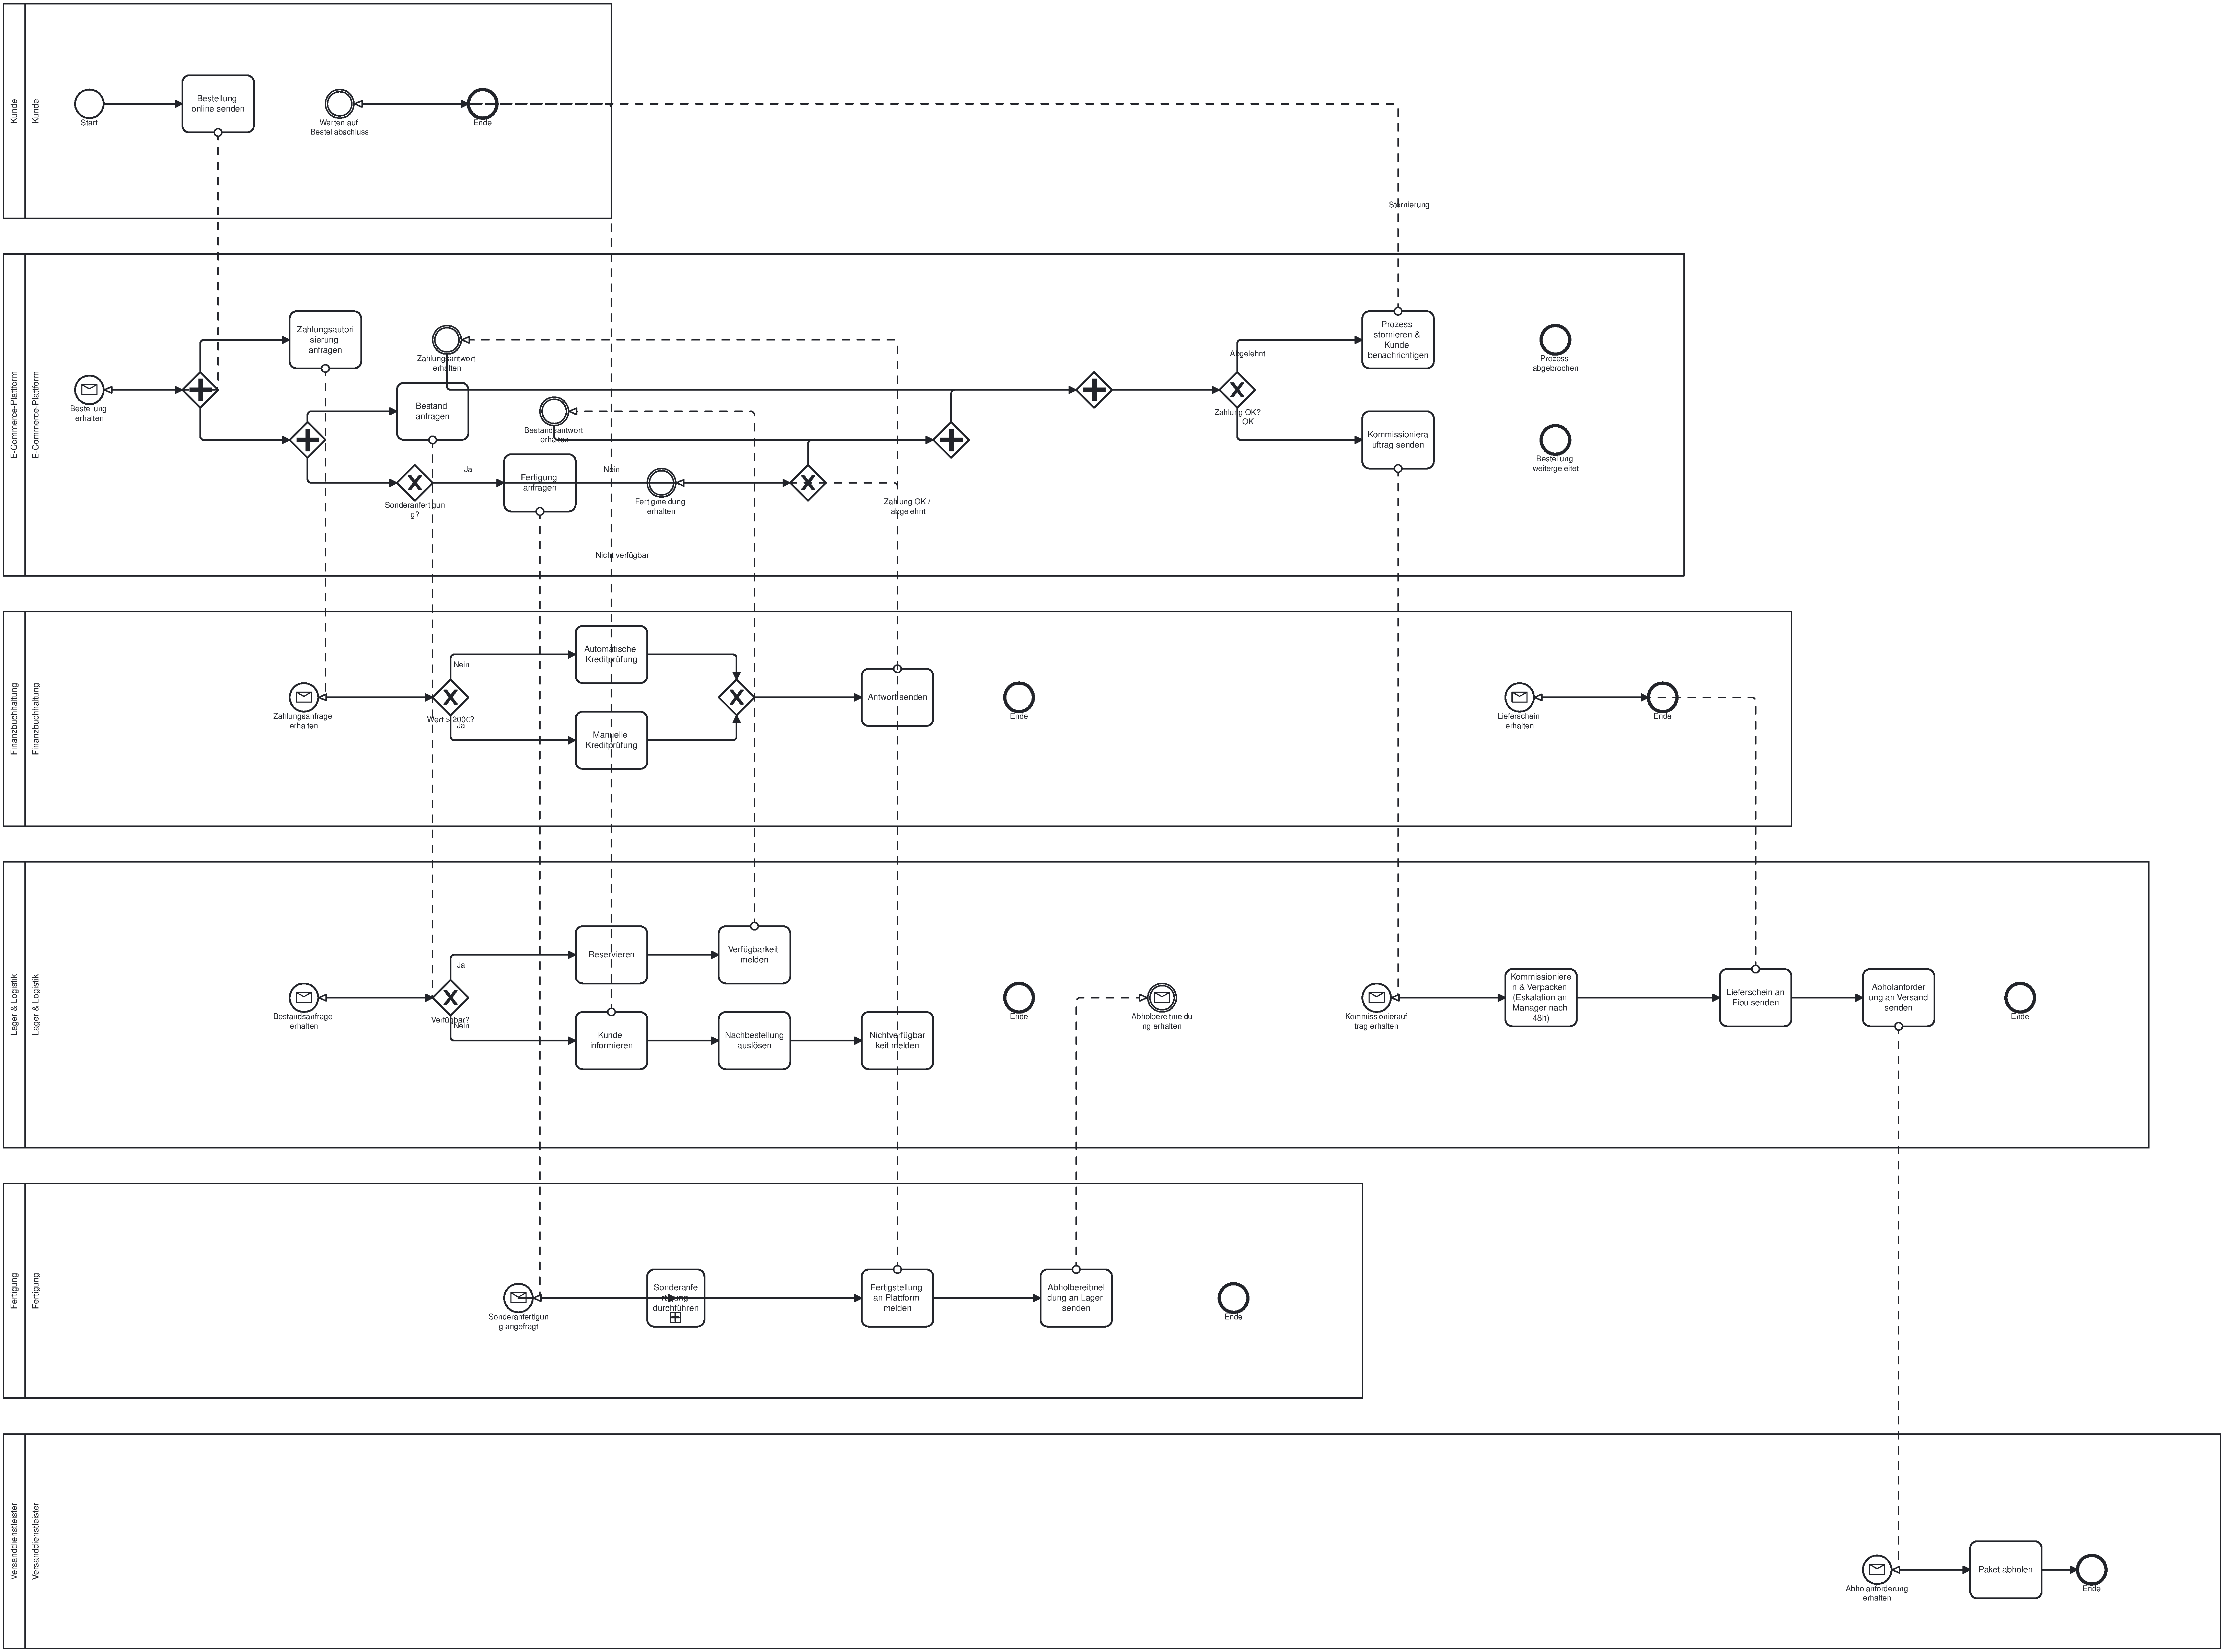
\includegraphics[width=\textwidth]{images/diagrams/gemini-2.5-pro-(json)-9zeuvovk}
  \caption{Diagramm von Gemini 2.5 Pro mit JSON}
  \label{fig:gemini-2-5-pro-json}
\end{figure}

\begin{figure}[!htb]
  \centering
  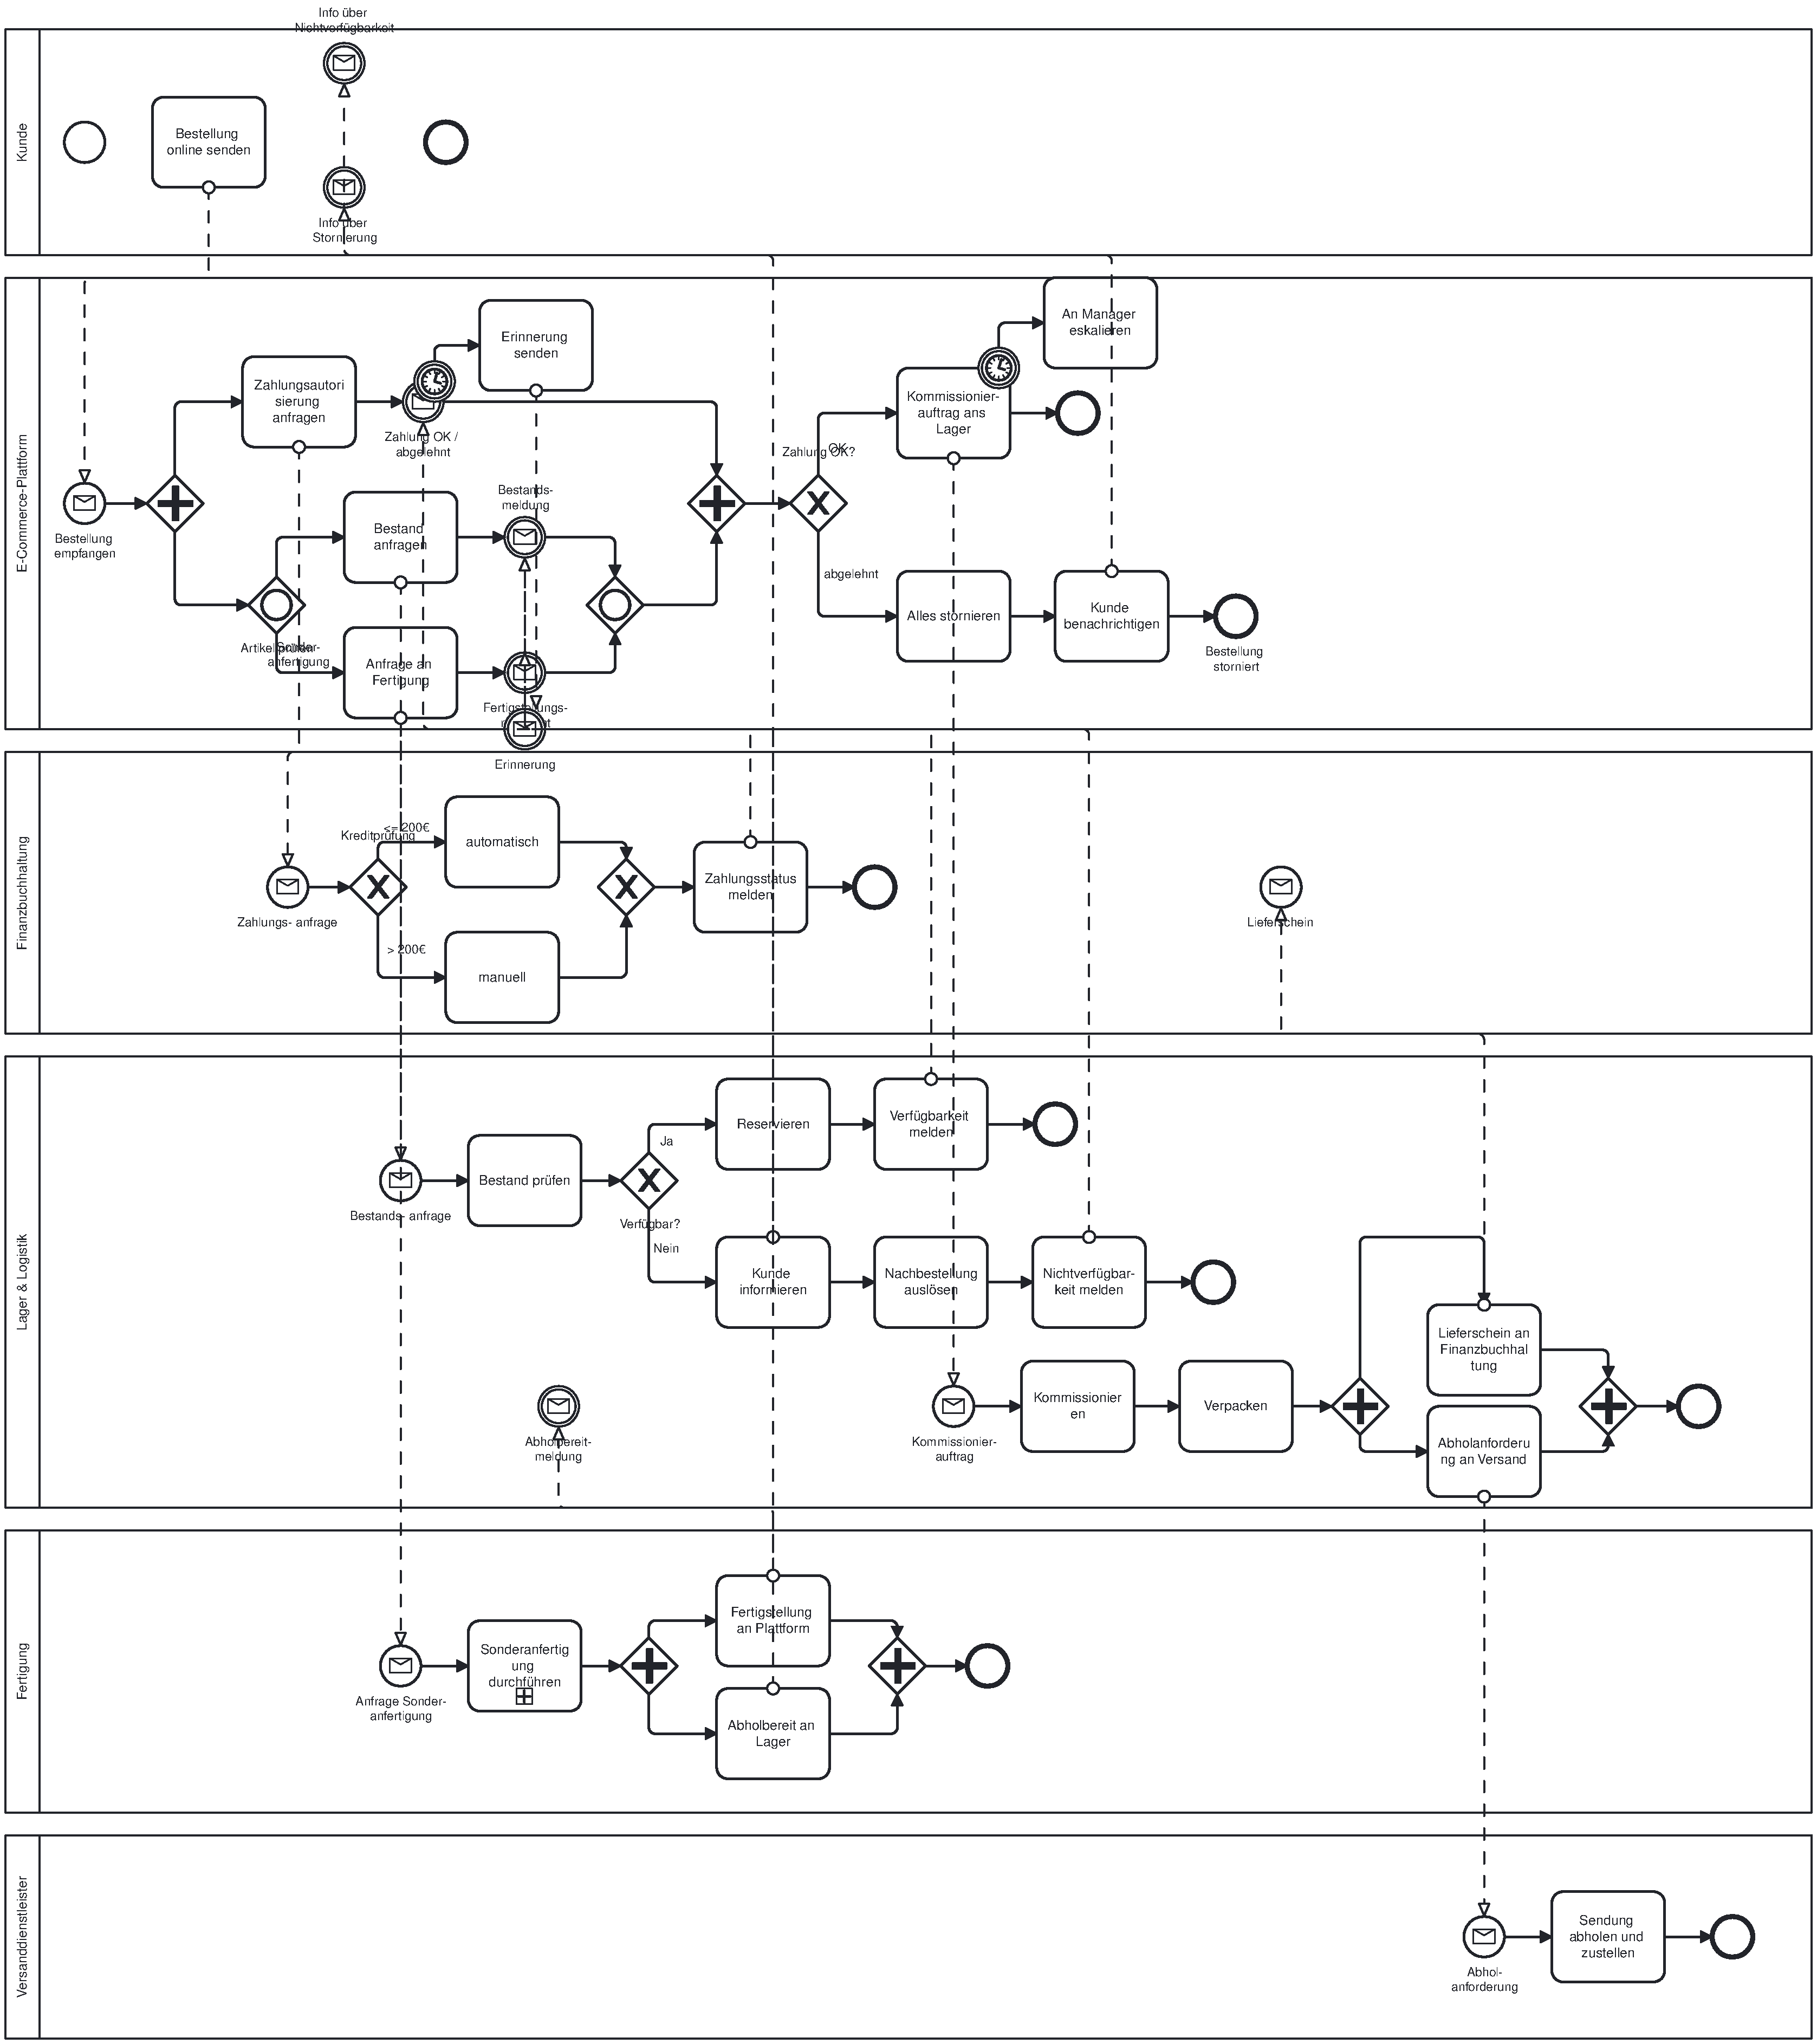
\includegraphics[width=\textwidth]{images/diagrams/gemini-2.5-pro-(xml)-67z0in69}
  \caption{Diagramm von Gemini 2.5 Pro mit XML}
  \label{fig:gemini-2-5-pro-xml}
\end{figure}

\begin{figure}[!htb]
  \centering
  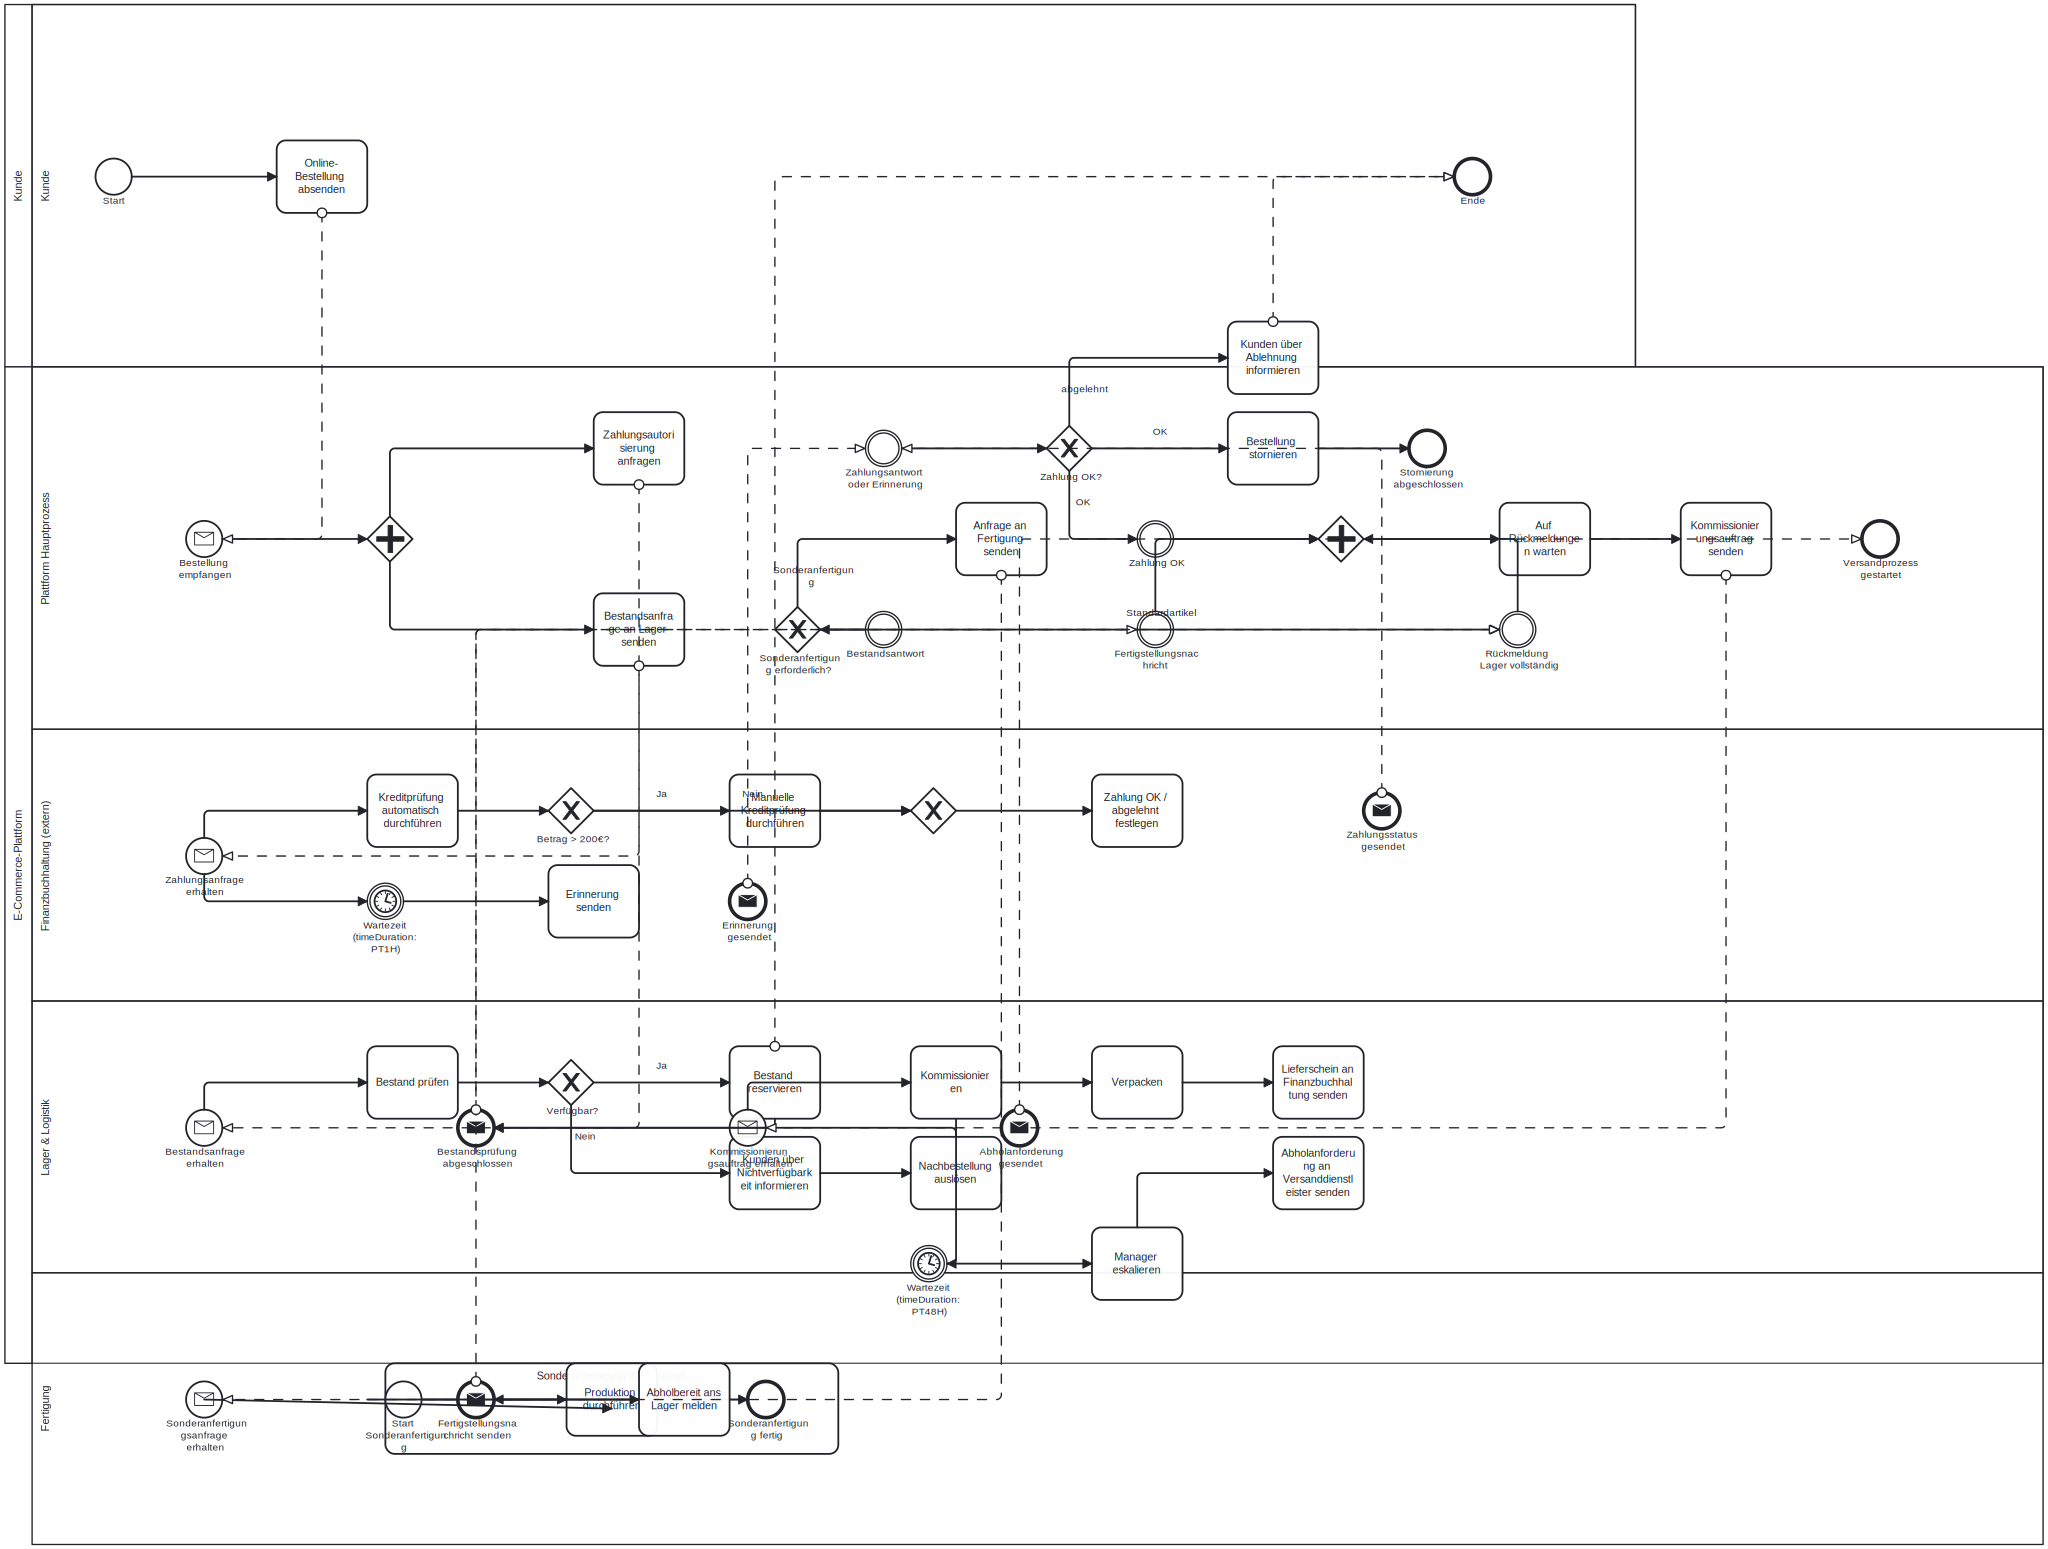
\includegraphics[width=\textwidth]{images/diagrams/gpt-5.1-(json)-ai2w4c2b}
  \caption{Diagramm von ChatGPT 5.1 mit JSON}
  \label{fig:gpt-5-1-json}
\end{figure}

\begin{figure}[!htb]
  \centering
  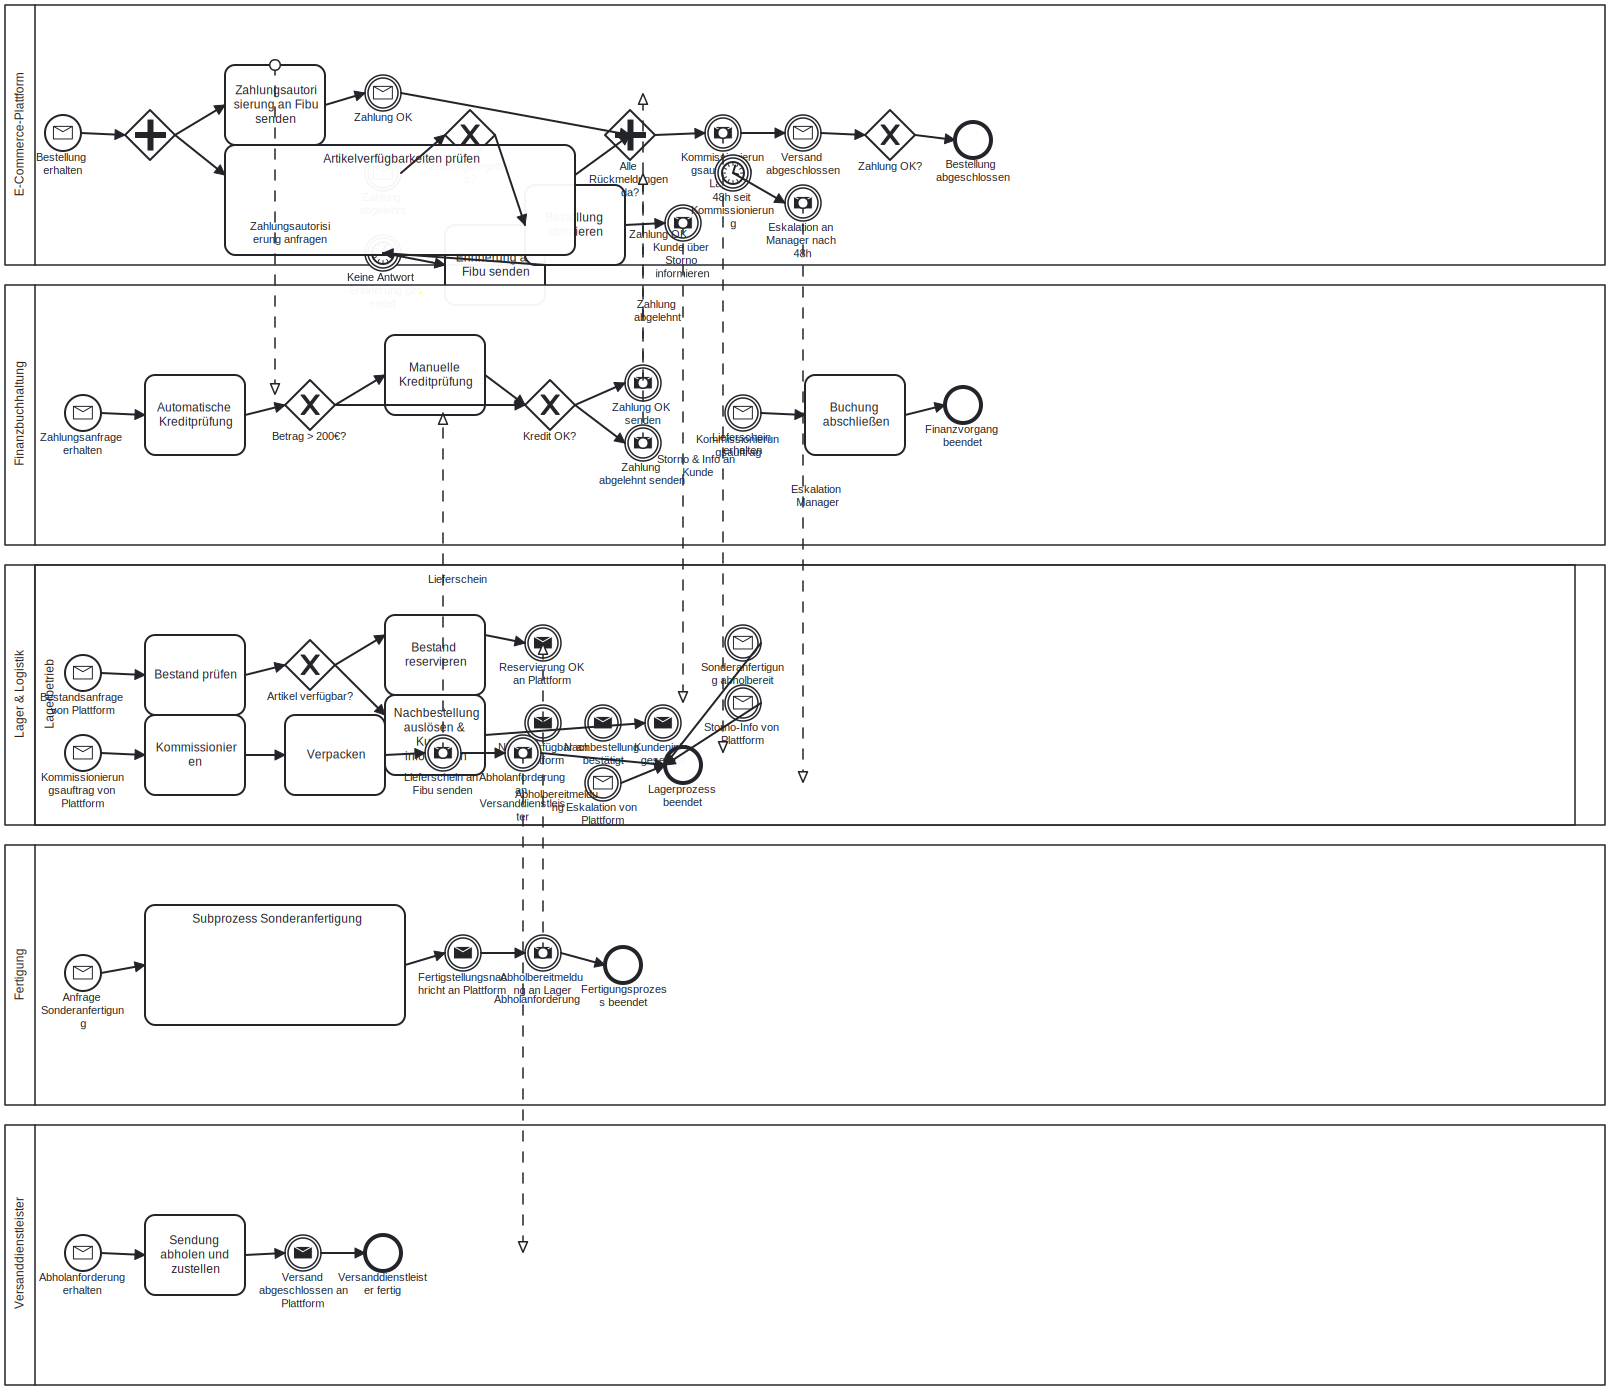
\includegraphics[width=\textwidth]{images/diagrams/gpt-5.1-(xml)-obl5u8o2}
  \caption{Diagramm von ChatGPT 5.1 mit XML}
  \label{fig:gpt-5-1-xml}
\end{figure}

\begin{figure}[!htb]
  \centering
  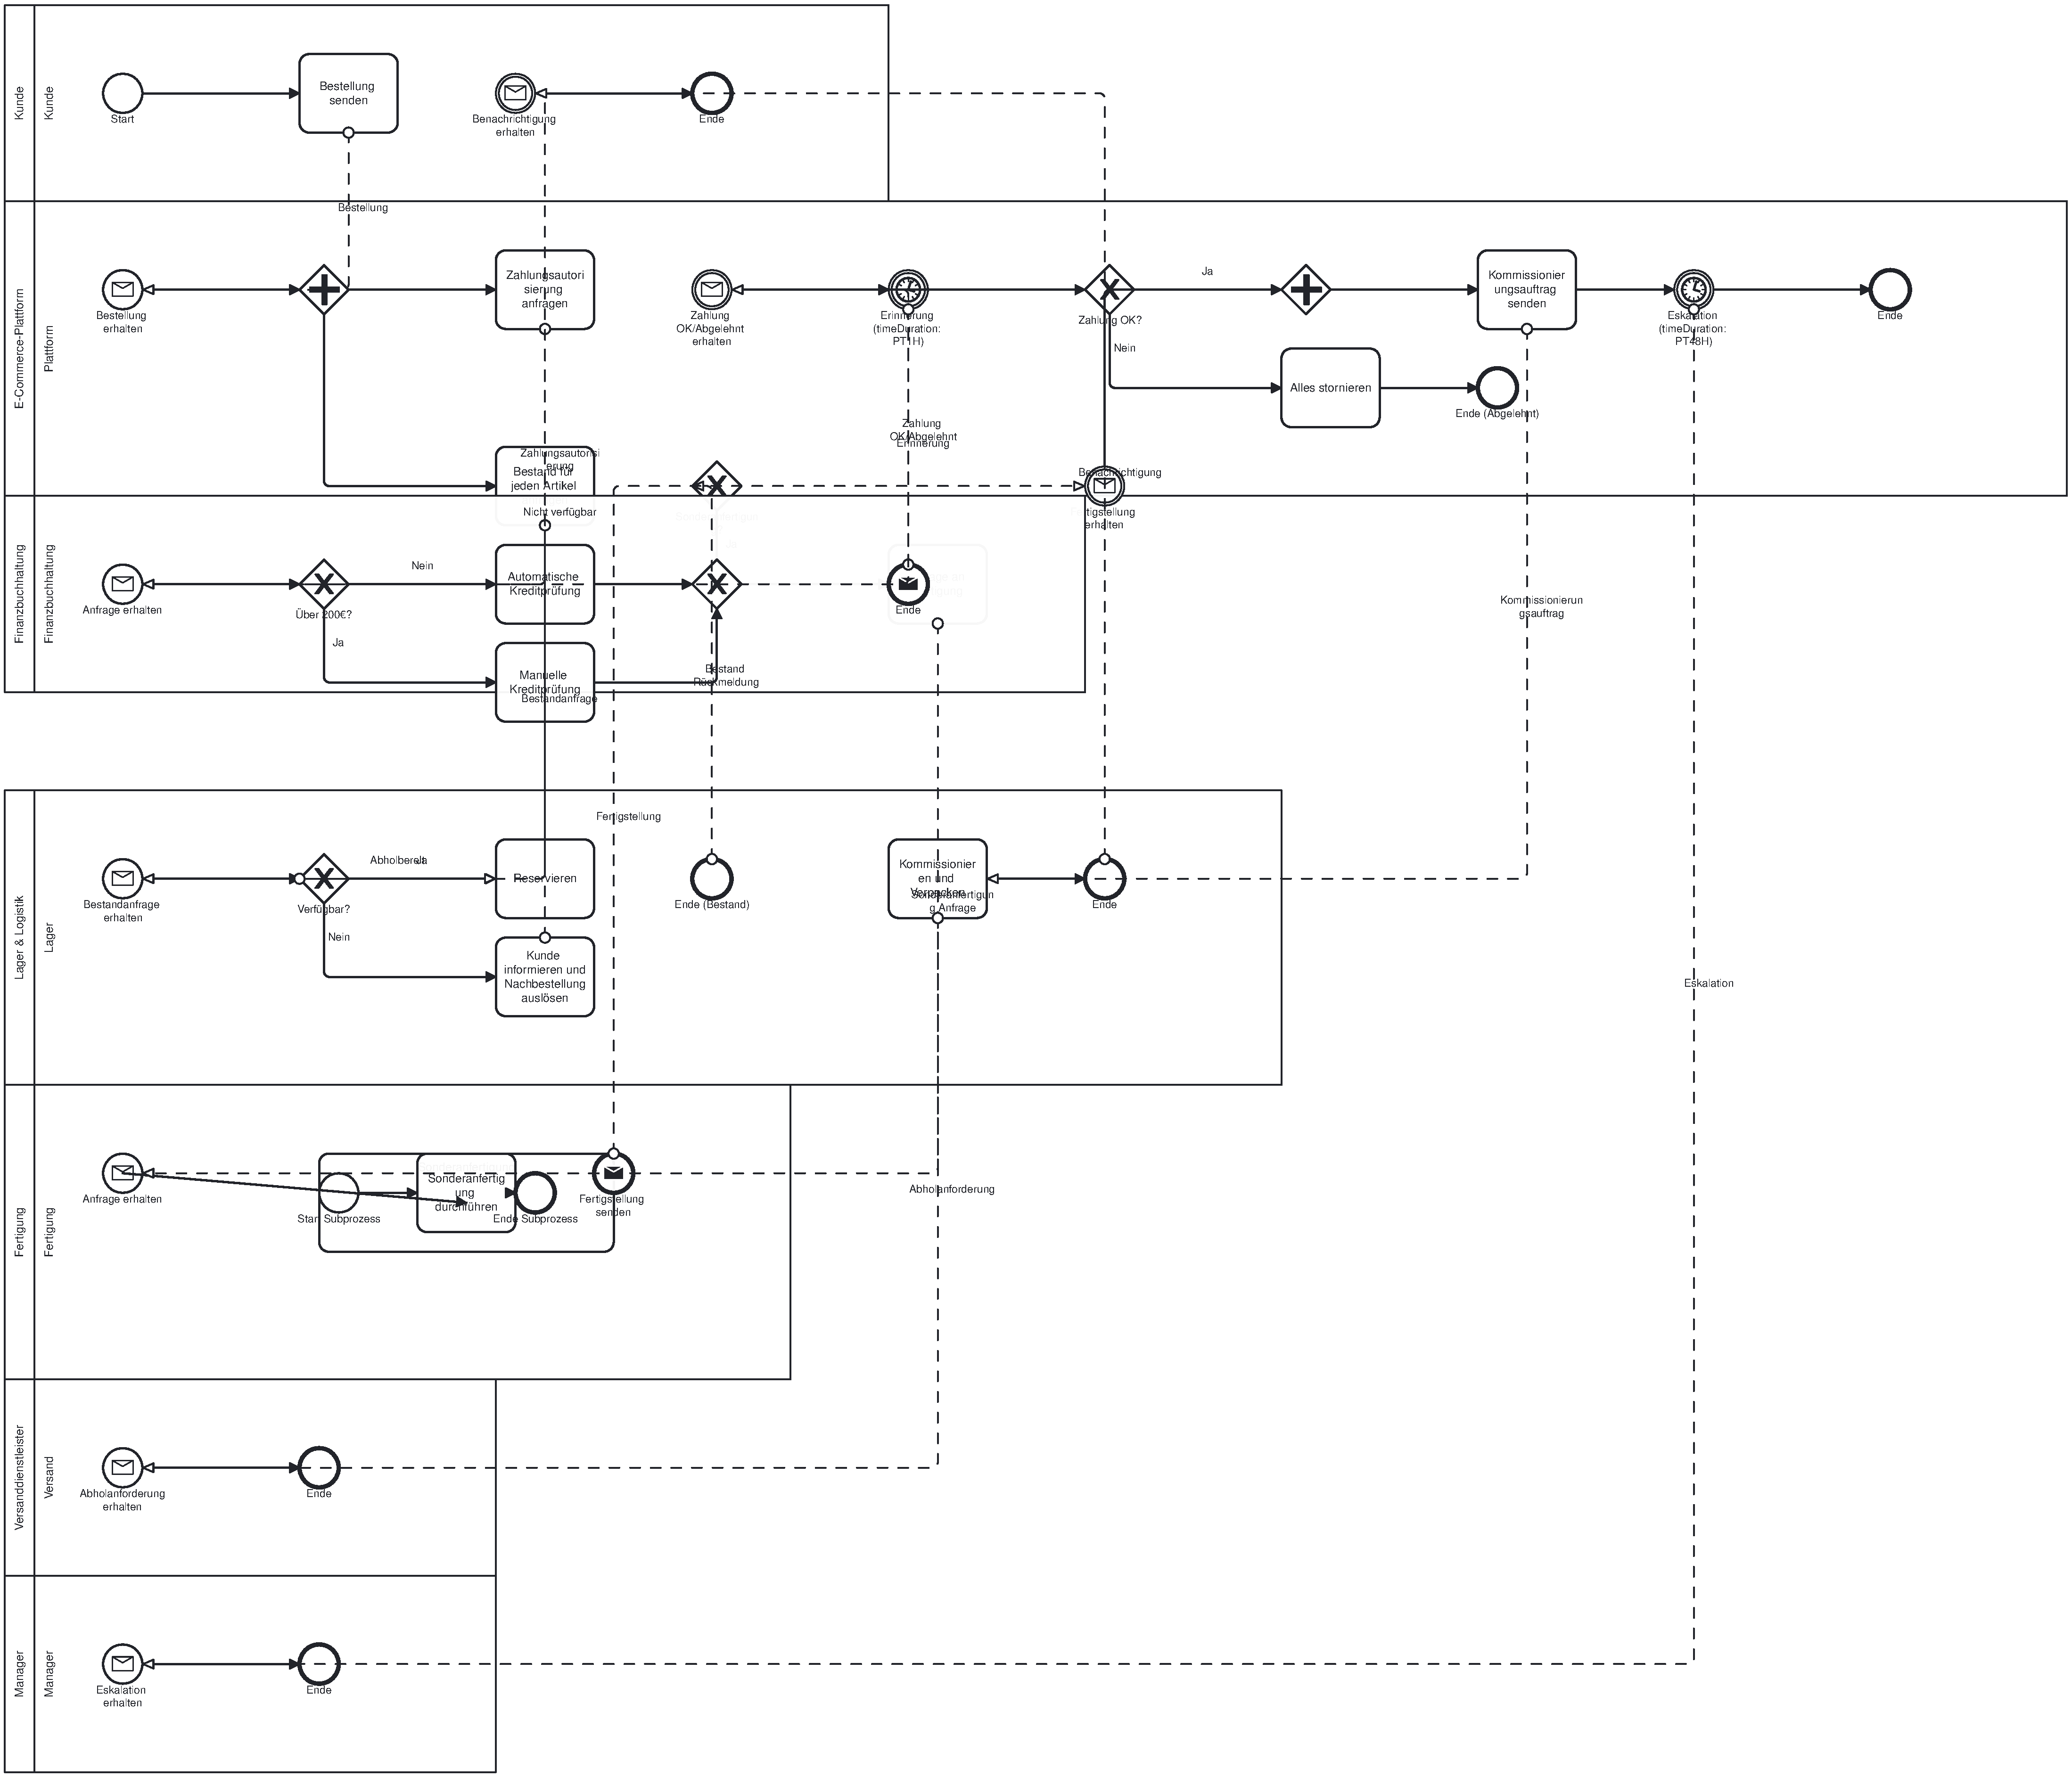
\includegraphics[width=\textwidth]{images/diagrams/grok-4-(json)-0pkdhn37}
  \caption{Diagramm von Grok 4 mit JSON}
  \label{fig:grok-4-json}
\end{figure}

\begin{figure}[!htb]
  \centering
  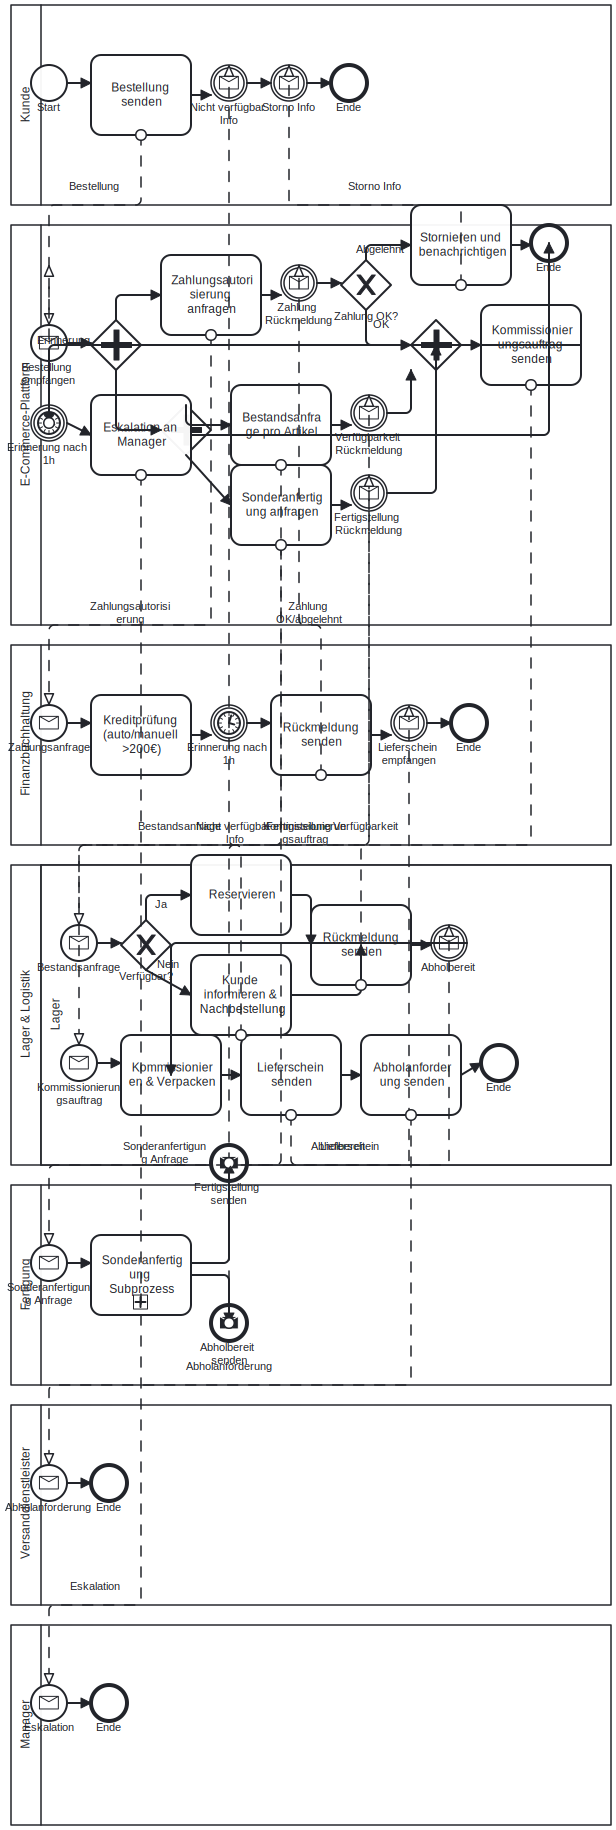
\includegraphics[height=.95\textheight]{images/diagrams/grok-4-(xml)-zyw3qofn}
  \caption{Diagramm von Grok 4 mit XML}
  \label{fig:grok-4-xml}
\end{figure}

\begin{figure}[!htb]
  \centering
  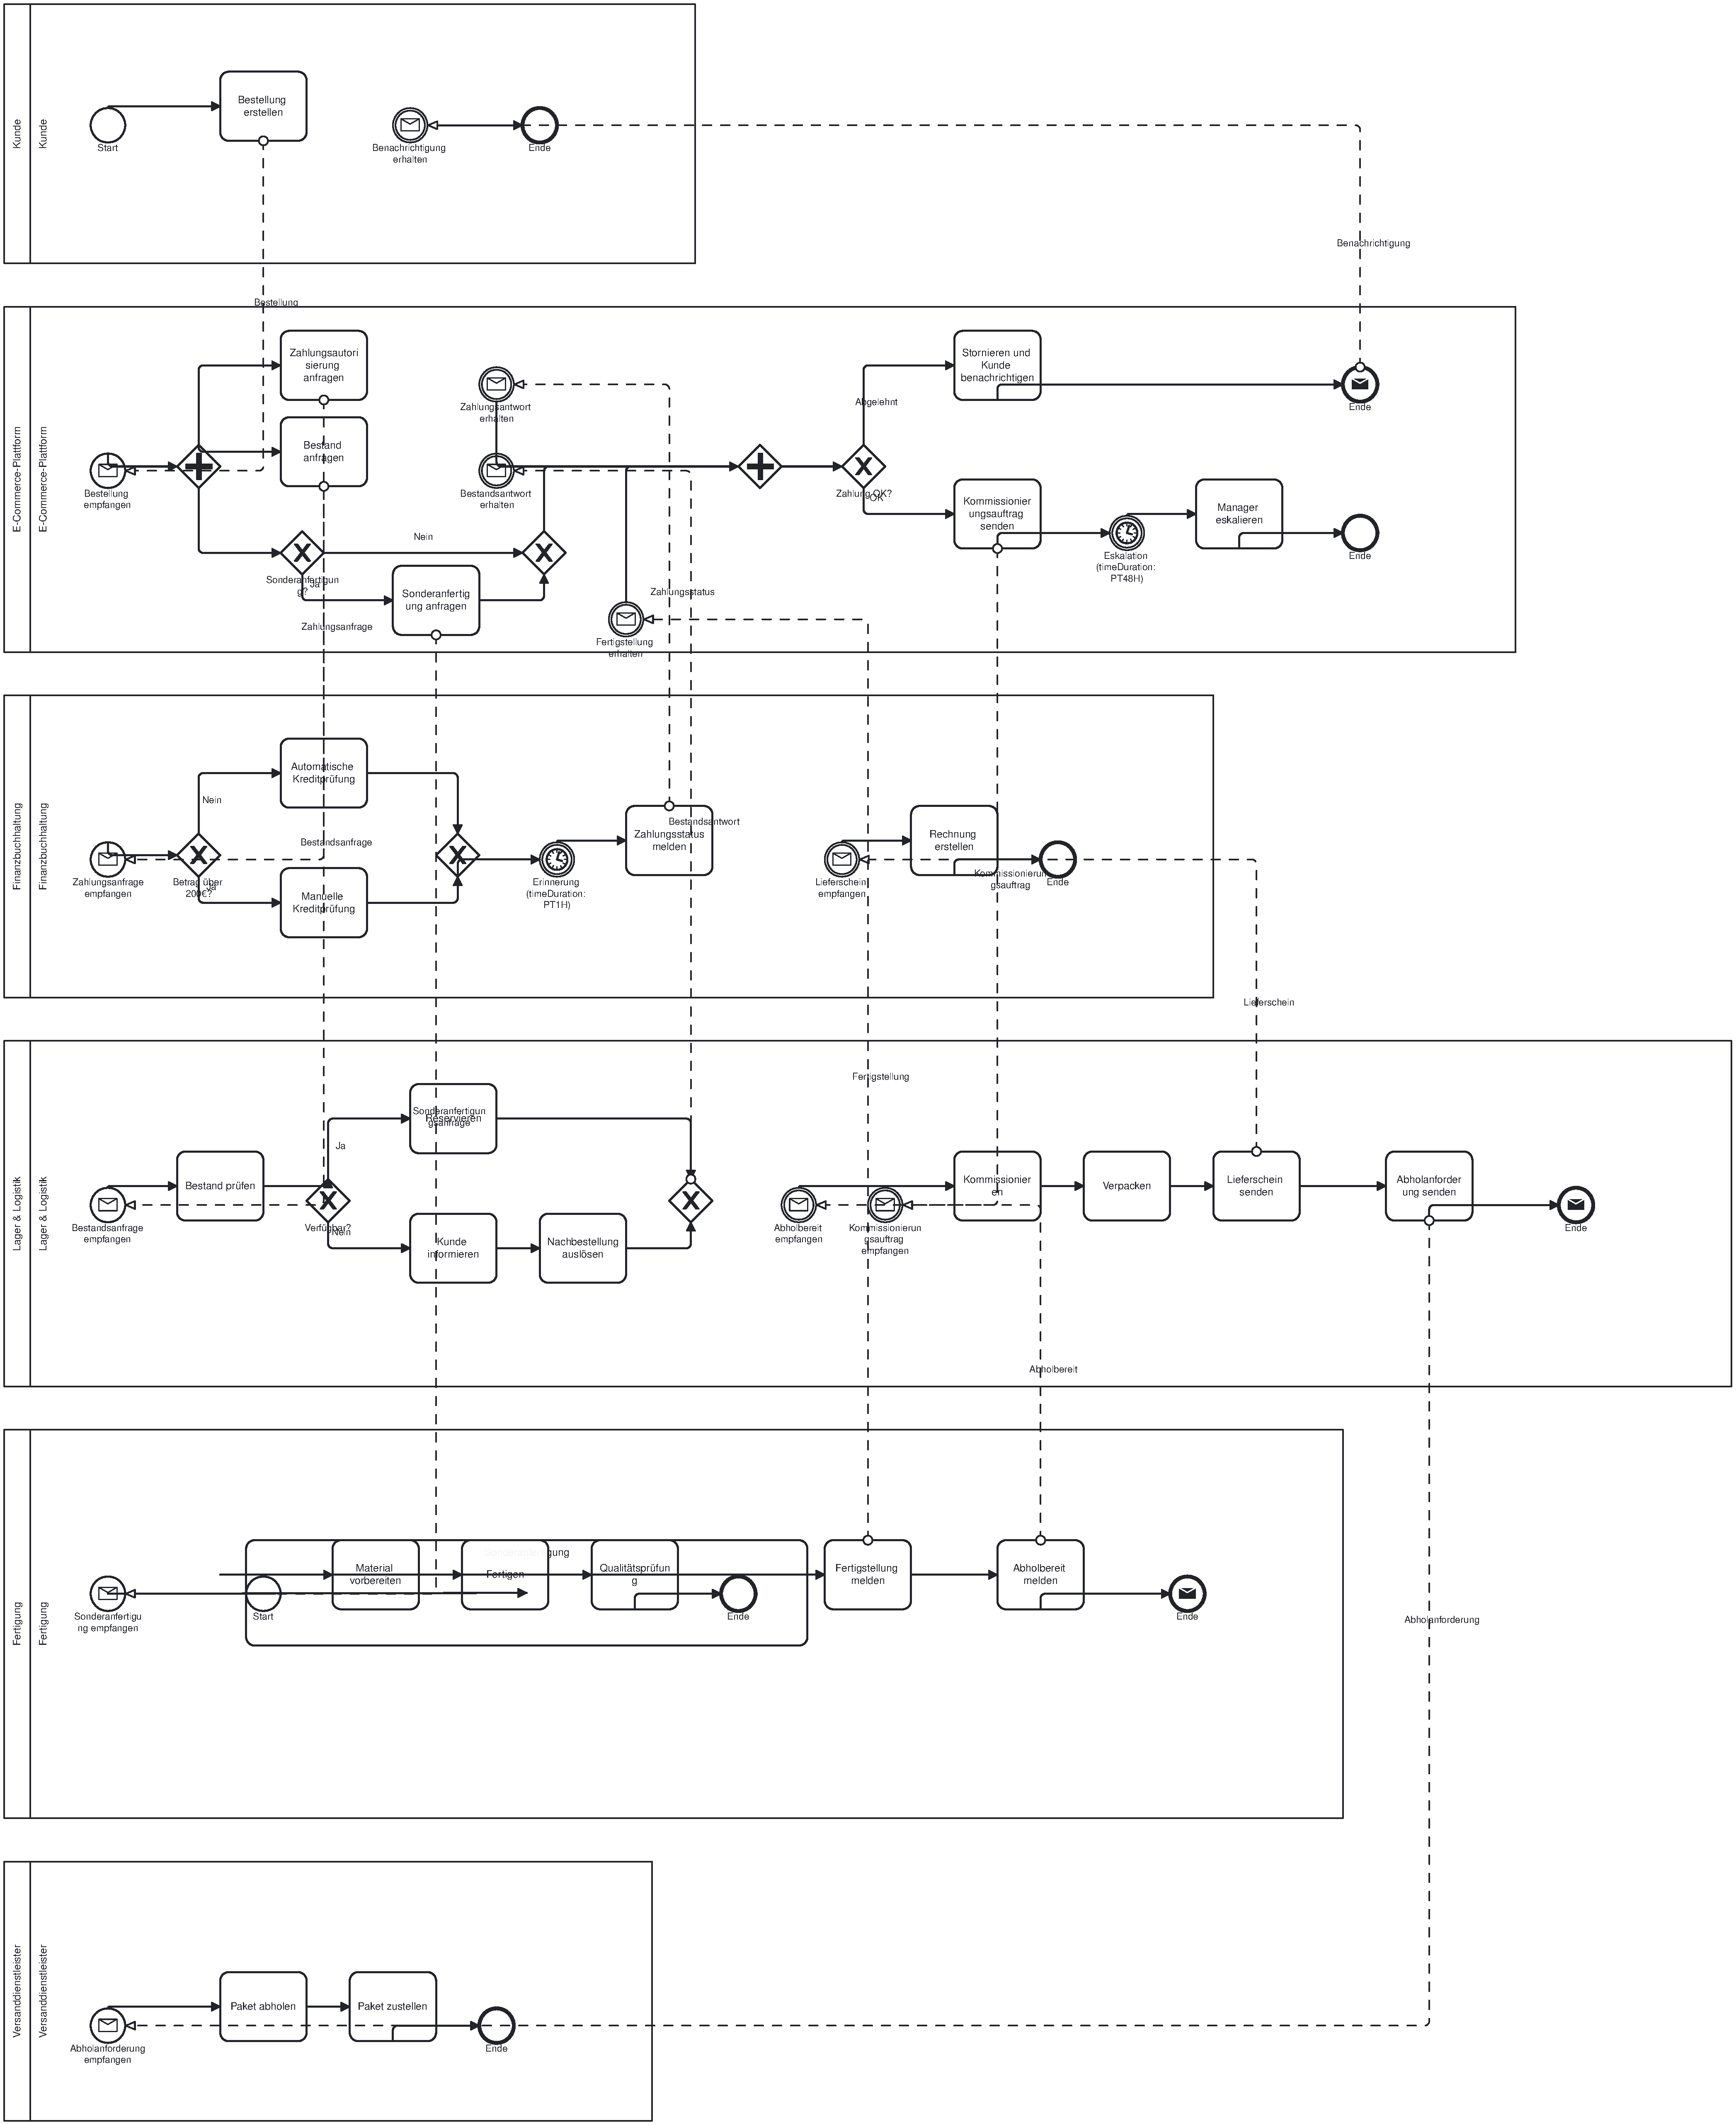
\includegraphics[width=\textwidth]{images/diagrams/claude-opus-4-5-(json)-p0ejrwf2}
  \caption{Diagramm von Claude Opus 4.5 mit JSON}
  \label{fig:claude-opus-4-5-json}
\end{figure}
